% !TEX program = xelatex
\documentclass{ctexart}
\usepackage{xcolor} % 在latex中使用颜色
\usepackage{booktabs,tabularx,multicol} % 制作表格
\usepackage{framed} % 制作文本框
\usepackage{amsmath,amsthm,amssymb,amsfonts}    % 数学符号与字体
\usepackage{hyperref}   % 添加超链接
\usepackage[left=2.0cm, right=2.0cm, top=2.5cm, bottom=2.5cm]{geometry} % 调整页边距
\usepackage{appendix}   % 附录环境
\usepackage{subfig,graphicx}    % 插入照片

%---------------优雅的插入MATLAB代码---------%
\usepackage{listings,matlab-prettifier} % MATLAB 美化包
\lstset{
        style=Matlab-editor,
        basicstyle=\mlttfamily,
        escapechar=`,
        numbers      = left,
        numbersep    = 5pt,
        numberstyle  = \small\color{red},
        frame        = single,
        keepspaces   = true,
        tabsize      = 4,
        breaklines = true,
}
%-------------标题-------------%
\author{}
\date{\today}
\title{三种求解微分方程数值解的方法}

%-----------做一些设置-----------%
\numberwithin{equation}{section}    % 公式标号与section的编号挂钩
\punctstyle{kaiming}    % 调整标点符号大小

%------------自定义一些命令------------%
\newcommand{\upcite}[1]{\textsuperscript{\textsuperscript{\cite{#1}}}}
\newcommand*{\dif}{\mathop{}\!\mathrm{d}}
\def\degree{${}^{\circ}$}

%---------配置环境------------%
\definecolor{shadecolor}{RGB}{241,241,255}
\newcounter{problemname}
\newenvironment{problem}{\begin{shaded}\stepcounter{problemname}\par\noindent\textbf{题目\arabic{problemname}. }}{\end{shaded}\par}
\newenvironment{solution}{\par\noindent\textbf{解答. }}{\par}
\newenvironment{note}{\par\noindent\textbf{题目\arabic{problemname}的注记. }}{\par}

%-------------可控列宽的表格--------%
\newcolumntype{R}[1]{>{\raggedright\arraybackslash}p{#1}}
\newcolumntype{C}[1]{>{\centering\arraybackslash}p{#1}}
\newcolumntype{L}[1]{>{\raggedleft\arraybackslash}p{#1}}

\usepackage{background}
\backgroundsetup{scale=2, angle=0, opacity = 0.5,contents = {
\includegraphics[width=\paperwidth, height=\paperwidth, keepaspectratio]{fig/背景.jpg}}}

\begin{document}
\maketitle
\tableofcontents
\newpage
\section{前言}
对于绝大多数微分方程,我们无法求出解析解。下面介绍三种针对问题
\begin{equation}
    y' = f(x,y)
\end{equation}
的求数值解的方法。
\section{欧拉法}
\subsection{算法公式}
\begin{equation}
    \begin{aligned}
        \omega_0 &= y_0\\
        \omega_{i+1} & = \omega_i + hf(t_i,\omega_i)\\
    \end{aligned}
\end{equation}
\subsection{代码示例}

\lstinputlisting[caption={\bf main.m},]{code/欧拉法/main.m}
\lstinputlisting[caption={\bf euler.m},]{code/欧拉法/euler.m}
\subsection{结果展示}

\begin{figure}[htp]
    \centering
    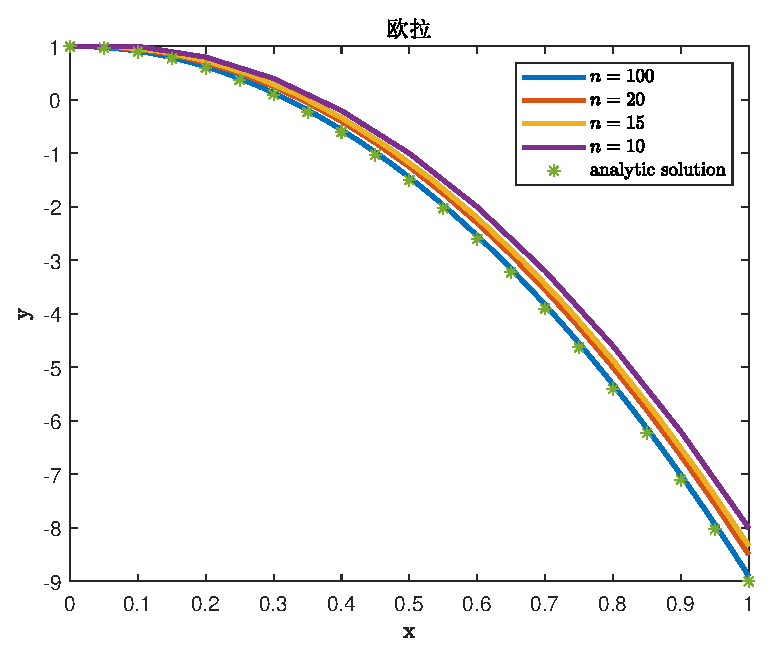
\includegraphics[width=0.7\linewidth]{fig/欧拉}
\end{figure}
可以看出,随着步长 $h$ 的不断减小,数值解也越来越精确。
\section{改进的欧拉法}
\subsection{算法公式}
\begin{equation}
    \omega_0 = y_0\\
    \omega_{i+1} = \omega_i + \frac{h}{2}(f(t_i,\omega_i)+f(t_i+h,\omega_i+hf(t_i,\omega_i)))\\
\end{equation}
\subsection{代码示例}
\lstinputlisting[caption={\bf main.m},]{code/改进欧拉法/main.m}
\lstinputlisting[caption={\bf euler\_improve.m},]{code/改进欧拉法/euler_improve.m}
\subsection{结果展示}
\begin{figure}[htp]
    \centering
    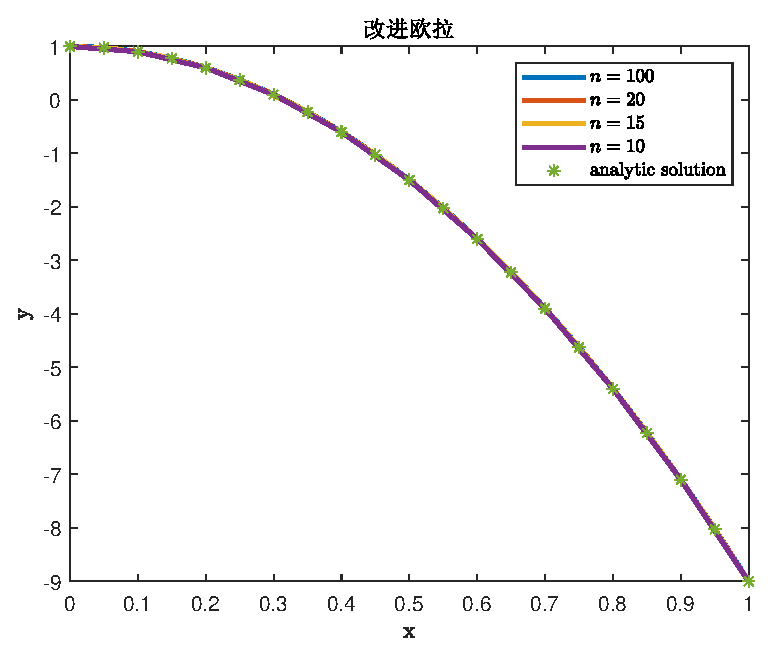
\includegraphics[width=0.7\linewidth]{fig/改进欧拉.eps}
\end{figure}
相比较于欧拉法,改进的欧拉在步长$h$较大时就已经取得了非常好的精度(以至于四条曲线几乎重合)。
\section{后退欧拉法}
\subsection{算法公式}
\begin{equation}
    \begin{aligned}
        \omega_0=y_0\\
        \omega_{i+1}=\omega_{i}+hf(t_{i+1},\omega_{i+1})
    \end{aligned}
\end{equation}
\subsection{代码示例}
\lstinputlisting[caption={\bf main.m},]{code/后退欧拉法/main.m}
\lstinputlisting[caption={\bf euler\_back.m},]{code/后退欧拉法/euler_back.m}
\subsection{结果展示}
\begin{figure}[htp]
    \centering
    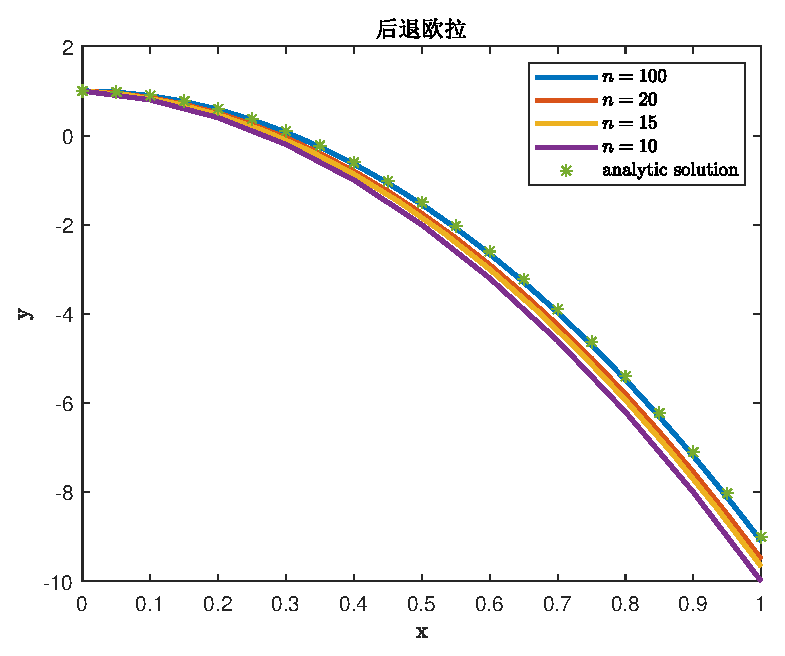
\includegraphics[width=0.7\linewidth]{fig/后退欧拉}
\end{figure}
后退欧拉法是一种隐式的方法,在编程过程中,需要利用迭代法来求解一个一元方程。相比较于显示方法,隐式方法允许在相对较大的步长中具有足够的误差控制,以及更好的效率。


\end{document}